\subsection{High Threshold Cherenkov Counter (HTCC)}

\subsection{Geometry}

The HTCC geometry is implemented through the native GEMC geometry API. The elliptical mirrors are made through a subtraction of
two G4Ellipsoid. They are contained inside an HTCC mother volume made with a G4Polycone, see \F{htccGeometry}.
The faces of the PMT are the sensitive volumes, associated with the quartz-glass material and associated with the HTCC digitization routine.

The refractive index of the $CO_2$ and its transparency is included in the material optical properties and taken
into account during the Geant4 transportation of the photons.

The mirror and Winston cones reflectivity is associated with the mirror optical properties and are taken into
account and taken into account during the Geant4 transportation of the photons.

The quartz window PMT quantum efficiency are associated with the PMT face optical properties and are taken into account in
the digitization routine.


\begin{figure}
	\centering
	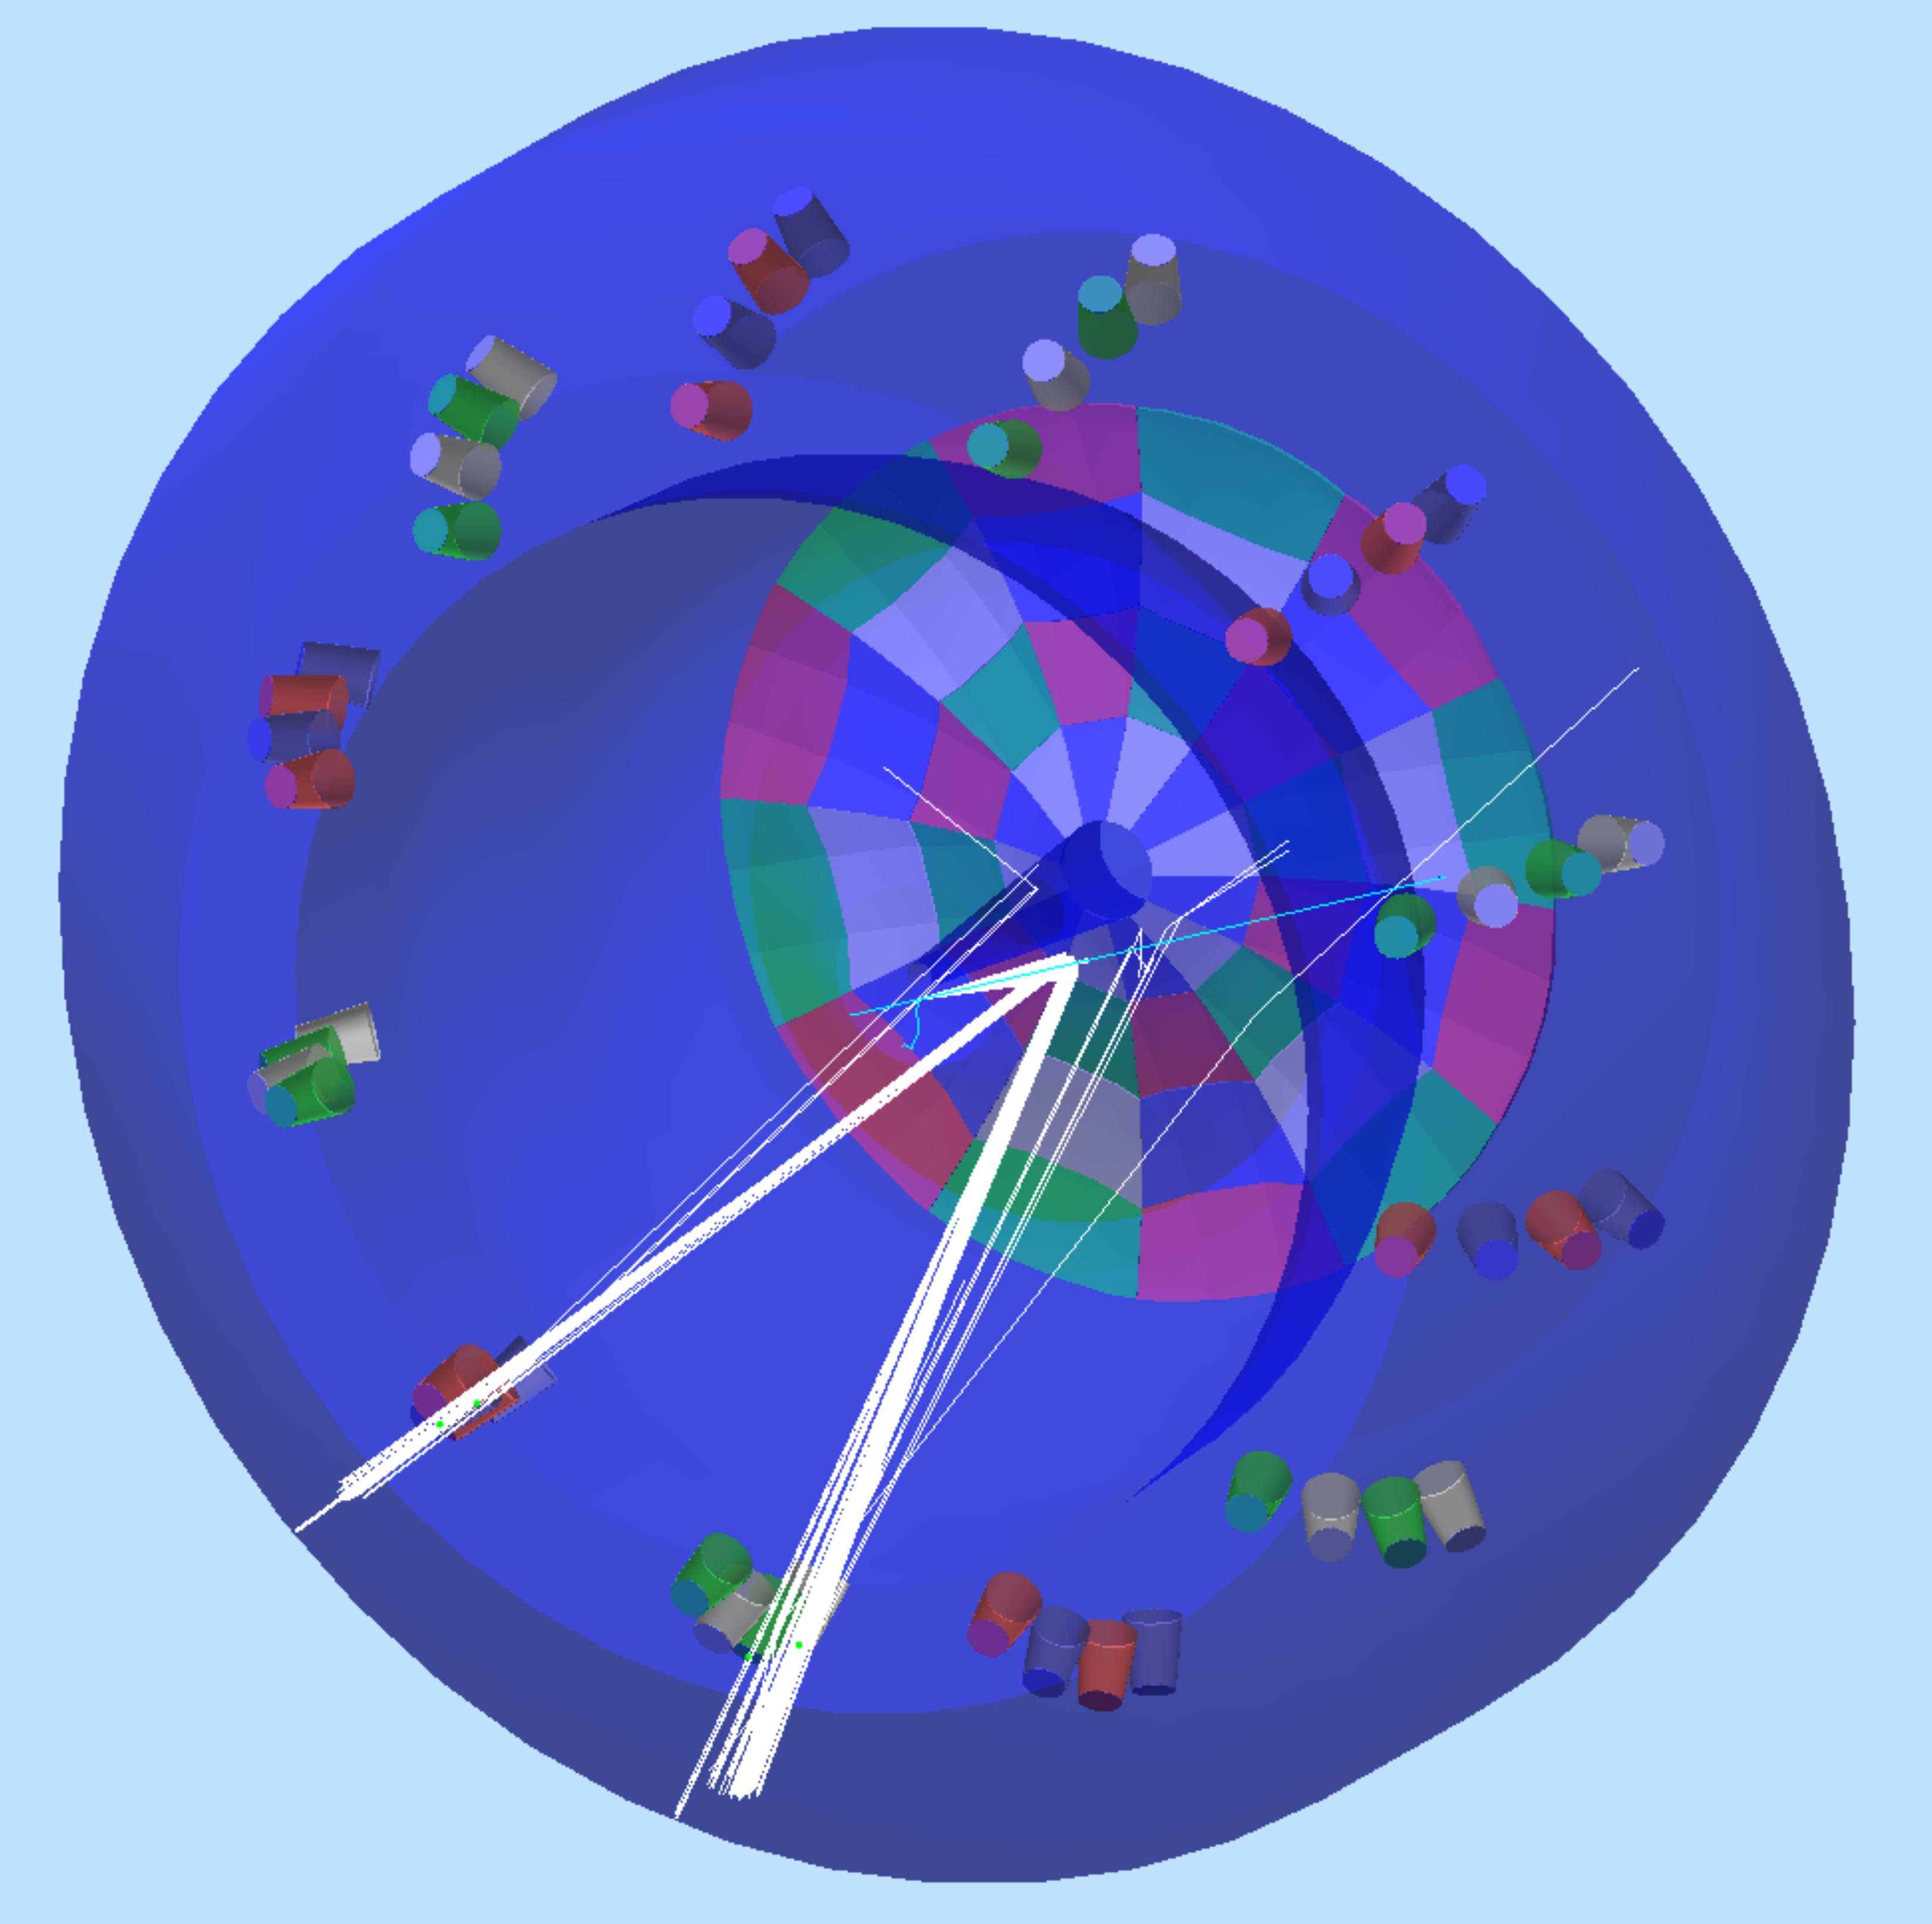
\includegraphics[width=0.99\columnwidth,keepaspectratio]{img/htccGeometry.png}
	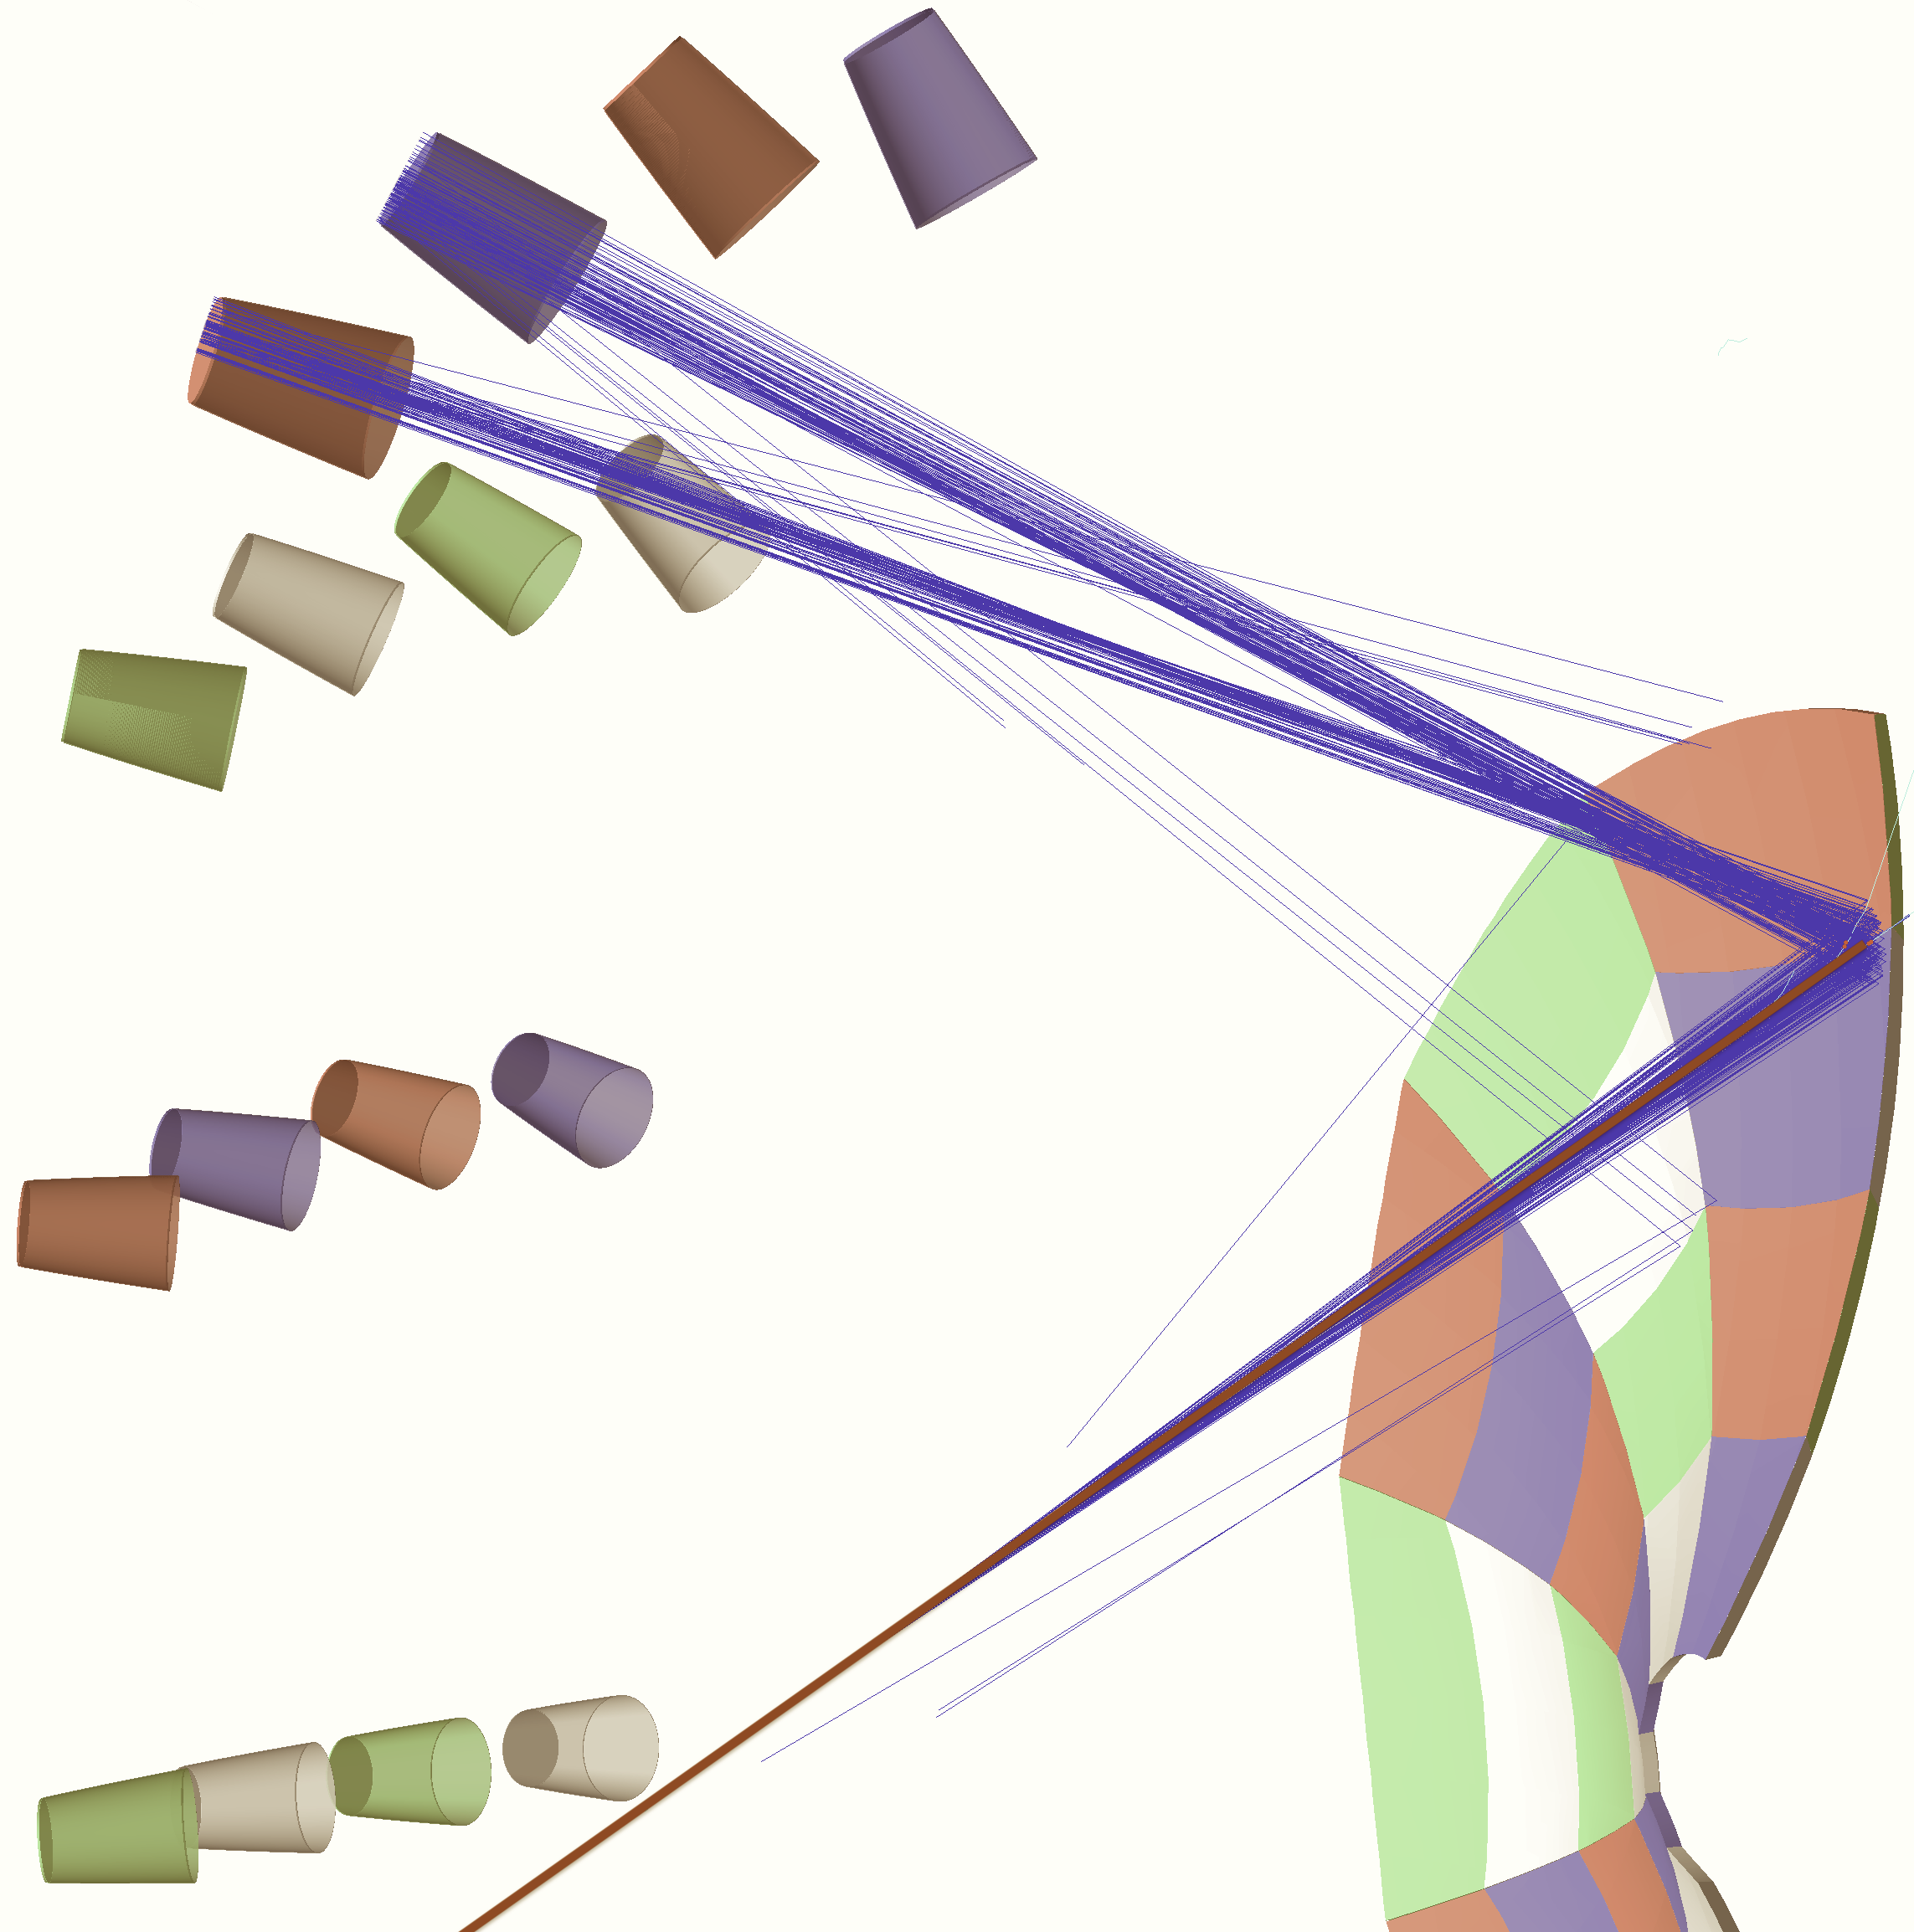
\includegraphics[width=0.99\columnwidth,keepaspectratio]{img/htccDetail.png}
	\caption{Top: an electron passing through the HTCC gas volume and emitting Cherenkov photons. The light cone
            hits two mirrors and it is re-directed to the corresponding PMTs.
            Bottom: details of the mirrors implementation. These are subtractions of ellipsoid Geant4 volumes along
            cetain planes between two adjacent mirror substrates. Each plane is defined by a second order
            curve along which the two substrates intersect. The curve is ``flat'', i.e. lies entirely in on that plane.}
	\label{fig:htccGeometry}
\end{figure}


The Github location of the GEMC perl API script is \url{https://github.com/gemc/detectors/tree/master/clas12/htcc}.



\subsection{Digitization}
Photons that impinged on the PMT faces are processed with the digitization routine.
For each photon collected undergoes the quantum efficiency algorithm at its wavelength to decided if it's finally detected.
The time average of all the photons is saved in the output after a time shift coming from the calibration database.
The digitized output bank variables are summarized in Table \ref{tab:htccBank}.

\begin{table}[h]
	\begin{center}
		\begin{tabular}{| c | c | c |}
			\hline \hline
			Variable         & Description    \\
			\hline
             sector &                                     clas12 sector     \\
             ring   &                                       theta index     \\
             half   &                                       half-sector     \\
             nphe   &                          number of photoelectrons     \\
             time   &                           average time of the hit     \\
             hitn   &                                        hit number     \\
			\hline \hline
		\end{tabular}
	\end{center}
	\caption{The digitized HTCC bank.}\label{tab:htccBank}
\end{table}

The time window  of the HTCC is set to 5 ns: all geant4 steps within the same PMT and time window will be collected on one hit.


The HTCC hit process routine location in git is \url{https://github.com/gemc/source/blob/master/hitprocess/clas12/htcc_hitprocess.cc}
